\chapter{抽樣分布與中央極限定理}
    我們在第三章中提到,做實驗或是抽樣時得到的結果具有隨機性,因此可以用隨機變數來代表,並用背後的機率分布來描述之。隨機變數的觀察值即為由其分布隨機抽出的\textbf{一個}數值。例如,那麼隨機抽取\textbf{一位}學生所得到的身高(以公分為單位)可以用隨機變數 $X$ 表示,且可以假定 $X$ 服從某個常態分布。然而,在實際收集及分析資料時,我們關注的通常不是一個觀察值,而是會抽取一組樣本並得到\textbf{一群}觀察值,並這群觀察值計算出我們有興趣的量。例如,我們可能抽出了 $50$ 位大學生測量身高,並計算他們的的身高平均值。這個平均值依然具有隨機性(抽出不同的同學,得到的平均身高就會不一樣),因此也可以用隨機變數來表示,例如 $\bar{X}$。此時如果我們要用這個身高平均值來做統計推論,就要了解 $\bar{X}$ 背後的機率分布為何。我們將在這章說明統計量抽樣分布的概念、樣本平均抽樣分布的性質,以及如何統計中最重要的\textbf{中央極限定理}來描述樣本平均的抽樣分布。
    
    \begin{introduction}[第 \thechapter 章學習目標]
        \item 了解抽樣分布的意義以及其與母體分布的不同
        \item 樣本平均抽樣分布的性質
        \item 中央極限定理的意義、適用範圍與應用
    \end{introduction}

\section{抽樣分布}
    假設清華大學的大學生身高服從一個平均值為 165 公分,標準差為 7 公分的常態分布。在前一章我們說過,如果把抽取一位學生得到的身高(以公分為單位)記作隨機變數 $X$,那麼我們可以寫作 $X \sim \NN(165, 7^2)$。這代表我們抽取一位學生測量身高時,相當於從 $\NN(165,7^2)$ 這個分布抽取一個數字。換句話說,如果我們重複地「抽取一位學生並測量身高」,那麼所得身高觀察值的分布將會如圖\ref{fig:sampling_mean}最左邊的直方圖。

    \begin{figure}[htbp]
        \centering
        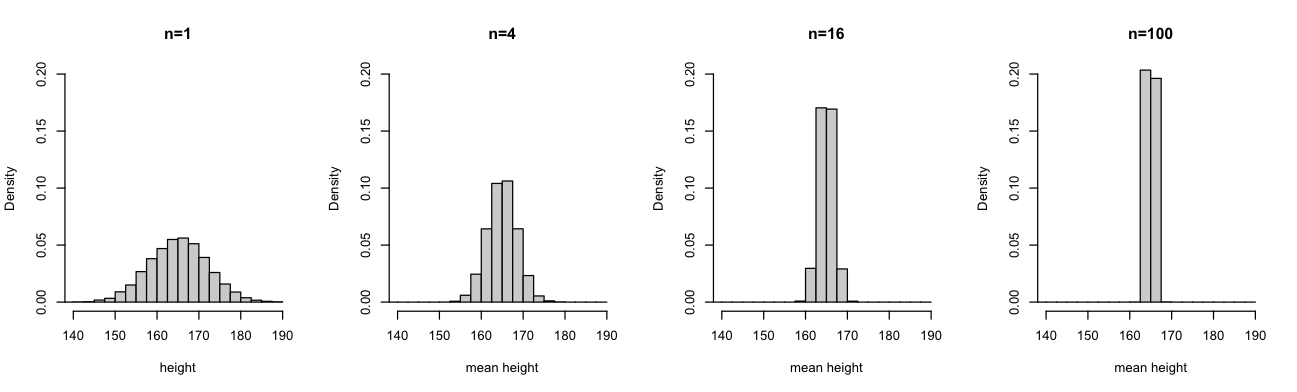
\includegraphics[width=\textwidth]{figures/04-Sampling_distribution_CLT/sampling_mean.png}
        \caption{身高平均值的抽樣分布}
        \label{fig:sampling_mean}
    \end{figure}

    現在假設我們隨機抽取了 4 位學生並測量身高。此時我們有 4 位學生,所以共有 4 個身高,但是這四個身高不能都用 $X$ 來表示(否則就隱含著四位學生身高均等),因此我們可以用 $X_1, X_2, X_3, X_4$ 來代表這 4 個身高對應的隨機變數。這 4 個隨機變數都服從 $N(165, 7 ^2)$ 的分配,而且互相獨立,所以我們可以寫作
    \[X_1 \sim \NN(165, 7^2)\;\; ; \;\;X_2 \sim \NN(165, 7^2)\;\; ;X_3 \sim \NN(165, 7^2)\;\; ;X_4 \sim \NN(165, 7^2)\;\;\]
    \[X_1,X_2,X_3,X_4\text{ 相互獨立 (mutually independent)}\]
    這種分布相同又相互獨立的情境在隨機抽樣中很常見,統計中給它一個專有名詞:\textit{獨立同分布} (independent and identically distributed),簡寫為 iid。因此,我們也可以寫為
    \[X_1, X_2, X_3, X_4 \overset{\text{iid}}{\sim} \NN(165, 7^2)\]
    此時如果我們計算身高的平均值並令其為隨機變數 $\bar{X}$,則 $\bar{X}$ 可以寫成:
    \[\bar{X} = \frac{X_1+X_2+X_3+X_4}{4}\]
    可以看到 $\bar{X}$ 是由樣本 $X_1,X_2,X_3,X_4$ 計算而得的隨機變數。這種不含未知參數、由樣本計算出的隨機變數在統計中被通稱為\textit{統計量} (statistic)。由於統計量是由隨機變數算出,它也會具有不確定性,也就是背後有一個分布。這個分布被稱為統計量的\textit{抽樣分布}(sampling distribution)。類似前面我們所說,我們抽取 4 位學生並算出平均身高時,相當於從 $\bar{X}$ 的抽樣分布抽取一個數字。換言之,如果我們重複地「抽取 4 位學生並計算平均身高」,所得平均身高的分布即為 $\bar{X}$ 的抽樣分布,如圖\ref{fig:sampling_mean}的左二直方圖。可以看到,\textbf{統計量的抽樣分布和樣本的機率分布是完全不一樣的},讀者一定要避免混淆。另外,如果我們不是抽取 4 位,而是抽取 16 位或 100 位學生來計算平均身高,則平均身高的抽樣分布如圖\ref{fig:sampling_mean}的右邊二個直方圖。可以看到,雖然都是平均值,但是抽取 4 位、16 位和 100 位學生計算出之平均值的抽樣分布都不一樣,因此樣本數也會影響統計量的抽樣分布。
    
    統計量的定義為「樣本計算出的隨機變數」,並不限於樣本平均,因此我們也可以建構其他統計量的抽樣分布:如果我們抽取 4 位、16 位或 100 位學生來計算身高樣本變異數,其抽樣分布則如圖\ref{fig:sampling_var}。可以看到這些抽樣分布均為右偏分布,和平均值的抽樣分布非常不同。總結來說,\textbf{統計量的種類和樣本數均可能影響抽樣分布的型態}。

    \begin{figure}[htbp]
        \centering
        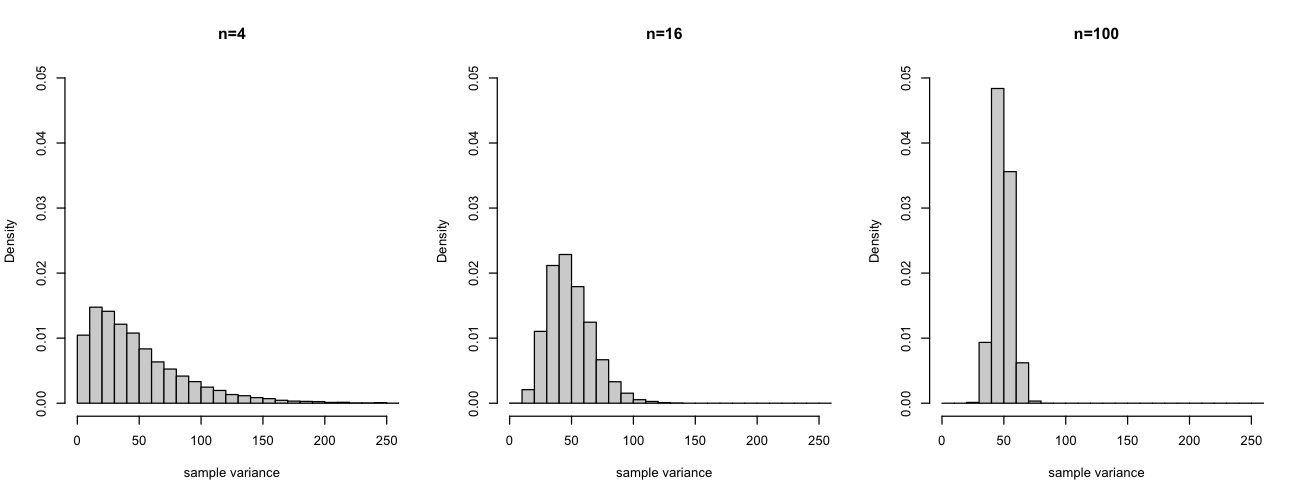
\includegraphics[width=\textwidth]{figures/04-Sampling_distribution_CLT/sampling_var.png}
        \caption{身高樣本變異數的抽樣分布}
        \label{fig:sampling_var}
    \end{figure}

    抽樣分布作為一個機率分布,也是可以計算期望值、變異數和標準差。其中統計量抽樣分布的標準差又被稱為統計量的\textit{標準誤} (standard error)。當統計量是用來估計母體參數時(例如樣本平均估計母體平均、樣本變異數估計母體變異數),統計量又被稱為\textit{估計量}(estimator),其觀察值則被稱為\textit{估計值} (estimate)。由於估計量具有變異性,估計值恰好等於母體參數的機會很低,但是我們可以藉由估計量的抽樣分布來考察估計值的表現。其中,估計量的期望值和標準誤是最直覺且重要的兩個評估點。
    
    如果估計量抽樣分布的期望值等於母體參數,代表估計值的取值會以母體參數為中心,我們就會比較信任這個估計量。這種估計量被稱為\textit{不偏估計量} (unbiased estimator)。例如在圖\ref{fig:sampling_mean}的左二圖中,如果我們用「四個學生的平均身高」作為清華大學生平均身高的估計量,可以看到這個估計量的抽樣分布平均值是 165,和母體平均相同,因此該估計量是不偏估計量。用符號來說,如果要估計的母體參數為 $\theta$,而我們提出的估計量是 $\hat{\theta}$,則 $\EE(\hat{\theta}) = \theta$ 時,$\hat{\theta}$ 為 $\theta$ 的不偏估計量。我們先前提到的樣本平均值、樣本變異數都是母體平均值、母體變異數的不偏估計量。

    估計量的標準誤代表了估計量取值的分散程度。當估計量為不偏時,雖然估計值雖然以母體參數為中心取值,但距離母體參數的遠近則不一定。例如圖\ref{fig:sampling_mean}中間的兩個圖中,「抽樣 4 位學生取身高平均」和「抽樣 16 位學生取身高平均」都是清華大學生身高平均值的不偏估計量,但是前者較可能出現 175, 155 這種偏離較多的估計值,後者則大多分布在 160 到 170 之間。因此,估計量的標準誤對於其估計精確程度也有影響。一般而言,我們希望估計量能夠不偏,又有很小的標準誤,這樣估計值就會非常接近母體參數。

    \bigskip
    
    \begin{custom}{思考}
        假設在清華大學生的例子中,我們抽樣 4 個人,並令 4 個人中最矮的人的身高為 $X_{(1)}$(以公分為單位)。請問 $X_{(1)}$ 是否為統計量?如何用重複抽樣的方式來畫出 $X_{(1)}$ 的抽樣分布?如果拿 $X_{(1)}$ 來估計清華大學生的平均身高,你覺得 $X_{(1)}$ 是否為不偏估計量?
    \end{custom}

    \bigskip

    \begin{custom}{思考}
        同樣是清華大學生的例子中,如果我們抽樣 100 個人並算出身高樣本變異數 A,然後再抽樣 250 個人並算出身高樣本變異數 B。那麼這兩個樣本變異數:(1) 都是估計母體的變異數,所以一般而言A、B數值會相近 (2) 是在估計平均值的標準誤,所以一般而言 A<B (3) 是在估計平均值的標準誤,所以後者一般而言 A>B。
    \end{custom}

    \bigskip

    \begin{custom}{思考}
        再次使用清華大學生的例子。如果我們隨機找一位學生,然後就用他的身高當成清華大學生平均身高的估計量。請問這個估計量是否為不偏估計量?
    \end{custom}
    
\section{樣本平均的抽樣分布}

    在各種統計量中,最常用的統計量就是樣本平均。因此,我們這裡針對樣本平均的統計性質作特別探討。假設我們從一個平均值為 $\mu$、變異數為 $\sigma^2$ 的母體抽出樣本數為 $n$ 的一組獨立樣本,得到的觀察值分別記為 $X_1, X_2, ..., X_n$。此時 $X_1, X_2, ..., X_n$ 為獨立同分布,期望值均為 $\mu$,變異數均為 $\sigma^2$。樣本平均可寫為
    \[\bar{X} = \frac{X_1 + X_2 + ... + X_n}{n} = \frac{1}{n}\sum_{i=1}^n X_i\]
    我們之前有學到隨機變數經過線性轉換後期望值和變異數的變化。我們來用這些先備知識來計算樣本平均的期望值。
    \begin{align*}
        \EE(\bar{X}) &= \EE\Big(\frac{X_1 + X_2 + ... + X_n}{n}\Big)&\\
        &= \frac{1}{n}\EE(X_1 + X_2 + ... + X_n)&\text{(縮放的期望值等於期望值縮放)}\\
        &= \frac{1}{n}[\EE(X_1) + \EE(X_2) + ... + \EE(X_n)]&\text{(相加的期望值等於期望值相加)}\\
        &= \frac{1}{n}[\mu + \mu + ... + \mu]&\text{(}X_i\text{獨立同分布,期望值為}\mu\text{)}\\
        &= \frac{1}{n}[n\mu] = \mu&\\
    \intertext{因此,\textbf{樣本平均是母體平均的不偏估計量}。接下來我們來計算樣本平均的變異數。}
        var(\bar{X}) &= var\Big(\frac{X_1 + X_2 + ... + X_n}{n}\Big)&\\
        &= \frac{1}{n^2}var(X_1 + X_2 + ... + X_n)&\text{(縮放的變異數等於變異數縮放平方倍)}\\
        &= \frac{1}{n}[var(X_1) + var(X_2) + ... + var(X_n)]&\text{(獨立隨機變數相加的變異數等於變異數相加)}\\
        &= \frac{1}{n}[\sigma^2 + \sigma^2 + ... + \sigma^2]&\text{(}X_i\text{獨立同分布,變異數為}\sigma^2\text{)}\\
        &= \frac{1}{n}[n\sigma^2] = \frac{\sigma^2}{n}&
    \end{align*}
    可以看到,\textbf{樣本平均的變異數是母體變異數除以樣本數}。把兩邊同時開根號後,我們得到
    \[sd(\bar{X}) = \frac{\sigma}{\sqrt{n}}\]
    因此,\textbf{樣本平均的標準誤是母體標準差除以根號樣本數}。因為樣本平均的標準誤太常用了,統計上給它一個專有名詞\textit{平均值標準誤} (standard error of the mean, SEM)。上述結果顯示,隨著樣本數增多,樣本平均對於母體平均的估計越來越精準,而且標準誤跟樣本數開根號呈反比。更進一步來說,當樣本數趨近於無窮大,平均值標準誤將會無限靠近零,也就是樣本平均會無限靠近母體平均。這個現象就是著名的\textit{大數法則} (Law of Large Numbers):只要樣本是獨立同分布,隨著樣本數增至無窮大,樣本平均終究會(機率)收斂至母體平均。

    注意到這裡我們在描述母體時,並沒有說它是什麼分布,而只說了它的平均值為 $\mu$、變異數為 $\sigma^2$。因此,母體分布是連續型或離散型、左偏右偏或對稱並不影響我們的結論。例如於圖\ref{fig:mean_dist_bern}中,我們假設母體為機率參數 0.64 的白努利分布,機率質量函數的型態如左上角。其平均值為 $0.64$,標準差為 $\sqrt{0.64*0.36} = 0.48$。右上、左下、右下分別是樣本數為 4、25、100 的樣本平均抽樣分布。其中可以看到樣本數為 4 時只有五種可能取值,因為樣本平均為四個白努利隨機變數的平均,也就是這四次白努力實驗成功次數除以 4,可能的取值就只有 0/4、1/4、2/4、3/4、4/4 這五種。圖中樣本平均抽樣分布的平均值均在 $0.6$,也就是白努利分布的平均值。標準誤則隨著樣本數增加而逐漸降低(分布逐漸變窄),且我們可以精確的算出各樣本數下的平均值標準誤。當 $n=4$ 時,標準誤應為 $\frac{0.48}{\sqrt{4}} = 0.12$、當$n=100$時,標準誤應為$\frac{0.48}{\sqrt{100}} = 0.048$。這種期望值不變,標準誤下降的現象在其他分布也同樣會出現,圖\ref{fig:mean_dist_unif}即用連續型的標準均一分布作為母體。

    \begin{figure}[htbp]
        \centering
        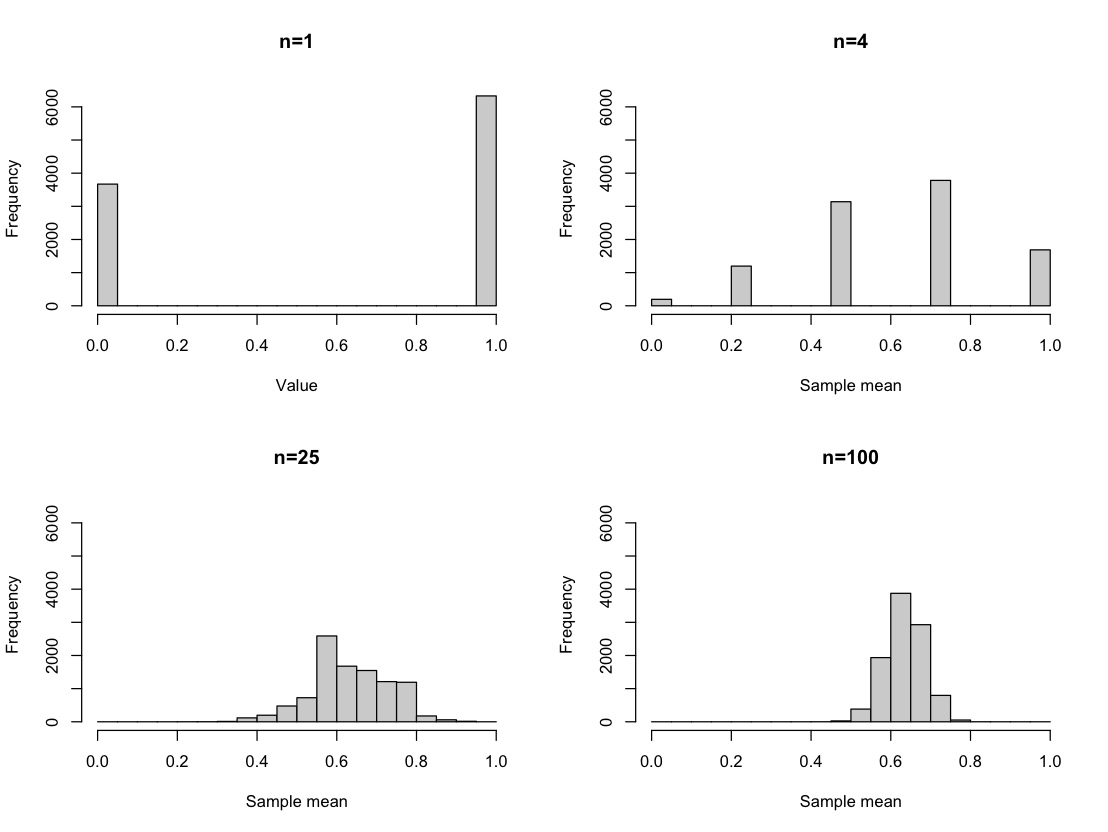
\includegraphics[width=0.9\textwidth]{figures/04-Sampling_distribution_CLT/mean_dist_bern.png}
        \caption{母體為 $Bernoulli(0.6)$ 的樣本平均抽樣分布}
        \label{fig:mean_dist_bern}
    \end{figure}

    \begin{figure}[htbp]
        \centering
        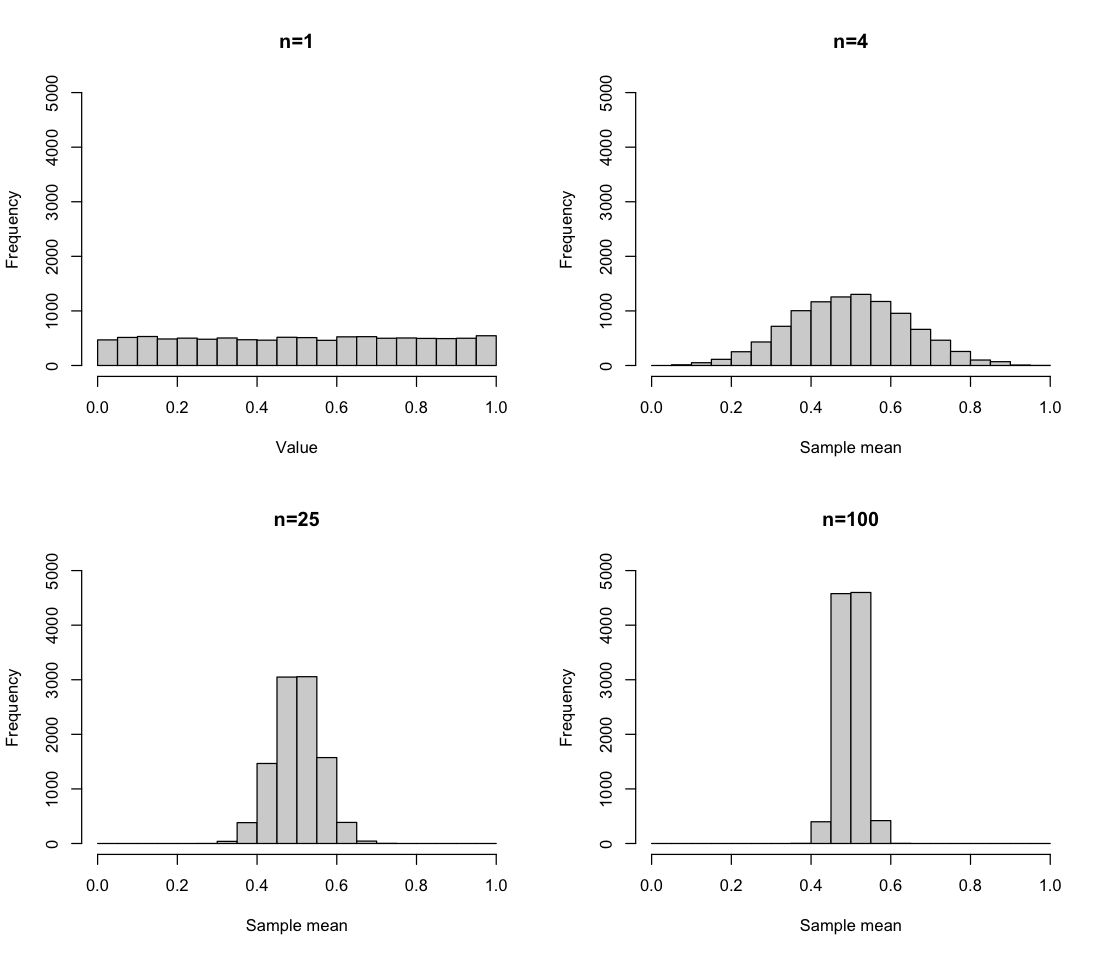
\includegraphics[width=0.9\textwidth]{figures/04-Sampling_distribution_CLT/mean_dist_unif.png}
        \caption{母體為標準均一分布的樣本平均抽樣分布}
        \label{fig:mean_dist_unif}
    \end{figure}

    一個特殊情況是,\textbf{當母體服從常態分布時,樣本平均也會服從常態分布}。由於常態分布只有兩個參數:平均值和變異數,而我們已知樣本平均的期望值是 $\mu$,變異數是 $\sigma^2/n$,所以我們可以直接寫出樣本平均的分布
    \[\bar{X} \sim \NN\Big(\mu, \frac{\sigma^2}{n}\Big)\]
    舉例而言,如果已知 60-70 歲男性的收縮壓 (mmHg) 分布服從 $\NN(130, 10)$ 的常態分布,那麼抽樣 16 位 60-70 歲男性算出的平均收縮壓就應該服從 $\NN(130, 10/\sqrt{16} = 2.5)$。我們還能依此算出平均收縮壓介於某個區間的機率,例如該平均收縮壓介於 125 至 135 mmHg 的機率為
    \[\PP(125 \le \bar{X} \le 135) = \PP\Big(\frac{125-130}{2.5} \le \frac{\bar{X}-130}{2.5} \le \frac{125-130}{2.5}\Big) = \PP(-2 \le \ZZ \le 2) \approx 0.954\]
    
    \bigskip

    \begin{custom}{練習}
        假設我們從平均值為 150 、標準差為 5 的母體抽出一個樣本數為 25 的樣本,則樣本標準差應該會最接近下列哪個數值:(1) 5 (2) 1 (3) 1/5。
    \end{custom}

    \bigskip

    \begin{custom}{練習}
        根據一項大型世代研究,45 歲以上氣喘患者的平均急性發作率為一年 0.22 次。假設一年氣喘的發作次數可用卜瓦松分布來描述。現由 45 歲以上氣喘患者中隨機抽取 100 人並計算他們平均一年氣喘發作的次數。該平均次數的期望值和標準誤應為何?
    \end{custom}

    \bigskip

    \begin{custom}{練習}
        回到清華大學生的例子。假設我們不知道清華大學生身高的分布,因此隨機抽取了三位學生來量身高,分別是 160、165、170 公分,並得到樣本平均值 165 公分以估計母體平均。請問我們是否知道該樣本平均的標準誤確切數值?若否,如何用資料來估計該樣本平均的標準誤?
    \end{custom}

    \bigskip

    \begin{custom}{思考}
        在醫學流病的應用研究中,通常會有製作一個 Table 1 來描述納入族群的特徵,例如性別比例、年齡、慢性病史比例等等。針對連續型變項例如年齡,假設樣本平均為 55 歲,樣本標準差為 10 歲,樣本數為 100 人,那麼年齡的敘述性統計應該寫成 $55 \pm 10$ (正負標準差)比較合理,還是 $55 \pm 1$ (正負標準誤)比較合理?
    \end{custom}
    
\section{中央極限定理}
    我們前面探討平均值抽樣分布的性質時,僅關注了它的期望值和標準差(即平均值標準誤),並且知道母體為常態分布時,樣本平均亦服從常態分布。然而,當母體非常態分布時,我們對於樣本平均的分布形狀並未著墨。觀察圖\ref{fig:mean_dist_bern}和\ref{fig:mean_dist_unif}可以看到,當樣本數比較少(n = 4, 25)的時候,平均值抽樣分布的型態較為取決於母體分布。例如母體為左偏的白努利分布時,平均值抽樣分布還是有點離散,而且大致上是左偏。不過當樣本數變大時(n = 100),兩個母體分布下的樣本平均抽樣分布都呈現大致對稱的鐘型。這個鐘型分布不是別的分布:正是常態分布!\textbf{不論母體分布為何},只要樣本數不斷增大,樣本平均抽樣分布都會趨近於常態分布。由於常態分布只有兩個參數:平均值與變異數,而我們在前一節已經導出樣本平均抽樣分布的平均值(母體平均)與變異數(母體變異數除以樣本數),所以這個趨近的常態分布就完全已知了。以上就是統計中最重要的\textit{中央極限定理} (Central Limit Theorem, CLT):

    \begin{theorem*}{(中央極限定理)}
        若 $X_1, X_2, ... X_n$ 為獨立同分布、平均值為 $\mu$、變異數為 $\sigma^2$ 的隨機變數,令樣本平均 $\bar{X} = \frac{1}{n}\sum_{i=1}^n X_i$,則當 $n \rightarrow \infty$
        \[\frac{\bar{X}-\mu}{\sigma/\sqrt{n}} \xrightarrow[]{d} \NN(0,1)\]
        或是用比較不嚴謹的寫法
        \[\bar{X} \xrightarrow[]{d} \NN\Big(\mu,\frac{\sigma^2}{n}\Big)\]
    \end{theorem*}
    中央極限定理精要就是\textbf{任何母體的樣本平均抽樣分布,在樣本「夠大」的情況下,會趨近於常態分布}。至於怎樣才叫「夠大」,理論上要視母體分布的偏斜和厚尾程度而定,但一般會認為樣本數大於 30 就足夠讓我們用常態分布來\textbf{近似}平均值抽樣分布。
    
    利用中央極限定理,我們就可以寫出更多估計量的近似分布,進而計算出估計量在指定區間的機率。例如,如果我們做一份 $n$ 人的民調,調查對於某議案的支持度,那麼每個民調受訪者是否支持其實都服從一個機率參數為 $p$ 的白努利分布,其中 $p$ 為全民對該議案的支持度。民調最後顯示的支持度 $\hat{p}$ 即為這些白努利分布隨機變數的平均值,因此根據中央極限定理,因為白努利分布的期望值為 $p$、變異數為 $p(1-p)$,我們有
    \[\hat{p} \xrightarrow[]{d} \NN\Big(p, \frac{p(1-p)}{n}\Big)\]
    因此,一個實際支持率為 $60\%$ 的議案,若做一份 $600$ 人的民調,其民調支持率 $\hat{p}$ 應趨近服從 $\NN(0.6, \frac{0.6 \cdot 0.4}{600} = 0.0004)$。根據這個近似抽樣分布,民調支持率低於 $55\%$ 的機率可以如下計算:
    \[\PP(\hat{p} \le 0.55) = \PP\Big(\frac{\hat{p}-0.6}{\sqrt{0.0004}} \le \frac{0.55-0.6}{\sqrt{0.0004}}\Big) \approx \PP(\ZZ \le -2.5) \approx 0.00621\]
    注意到如果我們把民調支持率乘上樣本數,就會得到支持人數。根據平均值與變異數的性質,支持人數 $Y$ 的近似分配可寫為
    \[Y = n\hat{p} \xrightarrow[]{d} \NN(np, np(1-p))\]
    先前我們提到過支持人數應該是遵從次數參數為 $n$、機率參數為 $p$ 的二項式分布,而這裡顯示支持人數在民調人數大時,趨進於上述的常態分布。這意味著二項式分布在次數參數 $n$ 足夠大的時候,可以用平均值與變異數相仿的常態分布來近似。至於怎樣叫作「足夠大」,一般認為 $np$ 和 $n(1-p)$ 均大於 $10$ 的時候近似效果就很好。同樣地,由於卜瓦松分布是二項式分布在 $np=\lambda$ 且 $n$ 趨近無限大時的分布,所以當 $\lambda > 10$ 時,我們也可以用 $\NN(\lambda, \lambda)$ 來近似卜瓦松分布。

    使用常態分布近似二項分布或卜瓦松分布時,為了讓近似更加準確,經常會引進\textit{連續性校正} (continuity correction),也就是把 $\PP(X = x)$ 的機率用常態分布中的 $\PP(x-0.5 \le X \le x + 0.5)$ 來近似。舉例來說,如果 $X \sim Poisson(36)$,且我們想計算 $32 \le X \le 37$ 的機率。因為速率參數已經大於 10,我們可以試著用 $\NN(36, 36)$ 來近似 $X$ 的分布。此時 $32 \le X \le 37$ 的機率,套用連續性校正後變成求 $31.5 \le X \le 37.5$ 的機率,因此計算如下
    \begin{align*}
        \PP(31.5 \le X \le 37.5) &= \PP\Big(\frac{31.5-36}{\sqrt{36}} \le \frac{X-36}{\sqrt{36}} \le \frac{37.5-36}{\sqrt{36}}\Big)\\
        &\approx \PP(-0.75 \le \ZZ \le 0.25) \approx (1-0.401)-0.227 = 0.372
    \end{align*}
    如果實際用卜瓦松分布的機率質量函數計算 $\PP(32 \le X \le 37) = \sum_{j=32}^{37} \frac{36^j e^{-36}}{j!} \approx 0.378$,可見近似的效果還不錯。除了用來作統計量的分布近似外,中央極限定理在推論統計的其他工具中扮演了舉足輕重的角色。我們會在未來的課程中不斷使用這個重要的定理。

    \bigskip

    \begin{custom}{練習}
        根據研究,服用降低血脂的 statin 類藥物出現嚴重肌病變的機率約為五千分之一。台灣的糖尿病與高血壓患者約有八萬五千人正在接受 statin 類藥物治療,試計算出現嚴重肌病變人數在 25 人以上的機率。
    \end{custom}

    \begin{docexam}{(107-2醫學(二))}
        下列何者不是中央極限定理的涵義?
        
        (A) 隨機樣本平均值之統計分布接近常態分布
        
        (B) 隨機樣本平均值之統計分布接近布阿松分布 (Poisson distribution)
        
        (C) 所有可能的隨機樣本平均值之平均值等於母群體平均值
        
        (D) 標準誤取決於母群體標準差與樣本的大小
    \end{docexam}

    \begin{docexam}{(105-2醫學(一))}
        下列對中央極限定理的描述,何者錯誤?
        
        (A) 只要樣本數夠大,無論原本母群體是否為常態分布,樣本平均值的抽樣分布會接近常態分布
        
        (B) 母群體的平均值若為 $\mu$,則樣本平均值抽樣分布的平均值為 $\mu$
        
        (C) 母群體的標準差若為 $\sigma$,則樣本平均值抽樣分布的標準差為 $\sigma/n$
        
        (D) 可透過中央極限定理將樣本平均值的抽樣分布變成標準常態分布
    \end{docexam}

    \begin{docexam}{(104-1醫學(一))}
        下列對中央極限定理的敘述,何者錯誤?
        
        (A) 只要樣本數夠大,樣本平均數的分布就會趨近常態分布
        
        (B) 只要樣本數夠大,樣本平均數分布的期望值就會很接近母體平均數
        
        (C) 只要樣本數超過 1,樣本平均數分布的標準差都會小於母體標準差
        
        (D) 母體分布只有在常態分布時,樣本數夠大時樣本平均數的分布才會趨近常態分布
    \end{docexam}

    \begin{docexam}{(103-2醫學(一))}
        一個等距尺度之臨床變數為雙峰分布,以大樣本經過多次重複抽樣之後,其樣本平均數的抽樣分布為一個常態分布。此現象反應下列何種定理?
        
        (A) 中央極限定理
        
        (B) 貝氏定理
        
        (C) 機率總和定理
        
        (D) 二項式定理
    \end{docexam}

    \begin{docexam}{(103-1醫學(一))}
        當樣本統計量與母群體母數之差的平均值為0,亦即統計量的期望值等於母數。此統計量具有下列何種統計學特性?
        
        (A) 有效性
        
        (B) 一致性
        
        (C) 充分性
        
        (D) 不偏性
    \end{docexam}

    \begin{docexam}{(102-2醫學(一))}
        下列對中央極限定理的敘述何者錯誤?
        
        (A) 樣本平均數之抽樣分布的標準差又稱標準誤,其值等於樣本標準差除以樣本數
        
        (B) 樣本平均數之抽樣分布的平均值等於母體平均值
        
        (C) 如果母群體為常態分布,即便樣本數不大,樣本平均數之抽樣分布也會接近常態分布
        
        (D) 如果樣本數夠大,則樣本平均數之抽樣分布定會接近常態分布
    \end{docexam}